\begin{figure}[!htb]
    \begin{centering}
        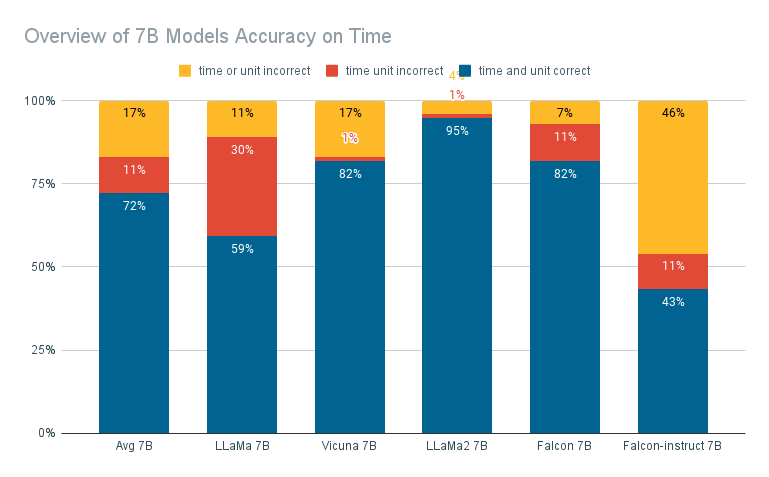
\includegraphics[width=\textwidth]{img/overview_7b_time}
        \caption[7B Models Detailed Time Accuracy]{\textbf{Detailed Overview of 7B Models Accuracy on Time.}
            On average, 7B sized models had an accuracy of 72\% on the extraction of the synthesis duration, and a third of the mistakes (11\% of 28\% total mistakes), were simply due to getting the unit of the duration wrong.
            \model{llama} struggled the most, providing inaccurate units for about a third of all answers on \ttime.
            Both \model{falcon} and \model{falcon}-instruct confused units in about 11\% of answers.
            However, \model{vicuna} and \model{llama2} gave the wrong unit in only 1\% of cases.
        }
        \label{fig:7b_time}
    \end{centering}
\end{figure}
